\documentclass[tikz,border=6pt]{standalone}

\usepackage{amsmath}
\usepackage{tikz}
\usetikzlibrary{arrows.meta,backgrounds,fit,positioning,calc}

\definecolor{RealGreen}{RGB}{104,183,120}
\definecolor{DummyGray}{RGB}{225,228,232}
\definecolor{MetaBlue}{RGB}{113,161,220}
\definecolor{HashOrange}{RGB}{245,176,65}
\definecolor{QueryPurple}{RGB}{155,89,182}
\definecolor{NoteGray}{RGB}{246,247,249}
\definecolor{PanelGray}{RGB}{250,250,251}

\tikzset{
  panel/.style={
    draw,
    rounded corners=5pt,
    fill=PanelGray,
    inner sep=7pt
  },
  title/.style={
    font=\scriptsize\bfseries
  },
  box/.style={
    draw,
    rounded corners=2.5pt,
    thick,
    align=center,
    minimum width=2.2cm,
    minimum height=0.62cm,
    fill=white,
    font=\small
  },
  mapbox/.style={
    draw,
    rounded corners=2.5pt,
    thick,
    align=left,
    minimum width=2.35cm,
    minimum height=0.72cm,
    fill=white,
    font=\scriptsize,
    inner sep=3.5pt
  },
  note/.style={
    draw,
    rounded corners=3pt,
    fill=NoteGray,
    align=center,
    inner sep=5pt,
    font=\footnotesize
  },
  arrow/.style={-Latex,thick}
}

\begin{document}
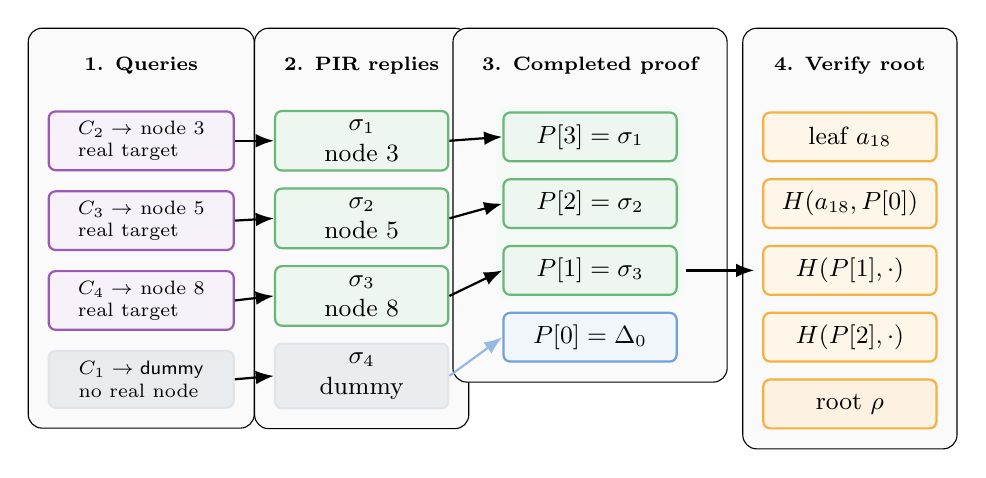
\begin{tikzpicture}[node distance=0.20cm and 0.45cm]

\node[title] (t0) at (1.45,4.9) {1. Queries};
\node[title] (t1) at (4.25,4.9) {2. PIR replies};
\node[title] (t2) at (7.15,4.9) {3. Completed proof};
\node[title] (t3) at (10.45,4.9) {4. Verify root};

\node[mapbox,draw=QueryPurple,fill=QueryPurple!8] (q1) at (1.45,3.95) {$C_2 \rightarrow$ node $3$\\real target};
\node[mapbox,draw=QueryPurple,fill=QueryPurple!8,below=0.24cm of q1] (q2) {$C_3 \rightarrow$ node $5$\\real target};
\node[mapbox,draw=QueryPurple,fill=QueryPurple!8,below=0.24cm of q2] (q3) {$C_4 \rightarrow$ node $8$\\real target};
\node[mapbox,draw=DummyGray,fill=DummyGray!72,below=0.24cm of q3] (q4) {$C_1 \rightarrow \mathsf{dummy}$\\no real node};

\node[box,draw=RealGreen,fill=RealGreen!12] (s1) at (4.25,3.95) {$\sigma_1$\\node $3$};
\node[box,draw=RealGreen,fill=RealGreen!12,below=of s1] (s2) {$\sigma_2$\\node $5$};
\node[box,draw=RealGreen,fill=RealGreen!12,below=of s2] (s3) {$\sigma_3$\\node $8$};
\node[box,draw=DummyGray,fill=DummyGray!70,below=of s3] (s4) {$\sigma_4$\\dummy};

\node[box,draw=RealGreen,fill=RealGreen!12] (p3) at (7.15,4.0) {$P[3]=\sigma_1$};
\node[box,draw=RealGreen,fill=RealGreen!12,below=of p3] (p2) {$P[2]=\sigma_2$};
\node[box,draw=RealGreen,fill=RealGreen!12,below=of p2] (p1) {$P[1]=\sigma_3$};
\node[box,draw=MetaBlue,fill=MetaBlue!10,below=of p1] (p0) {$P[0]=\Delta_0$};

\node[box,draw=HashOrange,fill=HashOrange!12] (h0) at (10.45,4.0) {leaf $a_{18}$};
\node[box,draw=HashOrange,fill=HashOrange!12,below=of h0] (h1) {$H(a_{18},P[0])$};
\node[box,draw=HashOrange,fill=HashOrange!12,below=of h1] (h2) {$H(P[1],\cdot)$};
\node[box,draw=HashOrange,fill=HashOrange!12,below=of h2] (h3) {$H(P[2],\cdot)$};
\node[box,draw=HashOrange,fill=HashOrange!16,below=of h3] (h4) {root $\rho$};

\draw[arrow] (q1.east) -- (s1.west);
\draw[arrow] (q2.east) -- (s2.west);
\draw[arrow] (q3.east) -- (s3.west);
\draw[arrow] (q4.east) -- (s4.west);

\draw[arrow] (s1.east) -- (p3.west);
\draw[arrow] (s2.east) -- (p2.west);
\draw[arrow] (s3.east) -- (p1.west);
\draw[arrow,draw=MetaBlue!75] (s4.east) -- (p0.west);

\draw[arrow] ($(p1.east)+(0.10,0)$) -- ($(h2.west)+(-0.10,0)$);

\begin{pgfonlayer}{background}
  \node[panel,fit=(t0)(q1)(q4)] {};
  \node[panel,fit=(t1)(s1)(s4)] {};
  \node[panel,fit=(t2)(p3)(p0)] {};
  \node[panel,fit=(t3)(h0)(h4)] {};
  \draw[draw=none,fill=RealGreen!7,rounded corners=5pt]
    ($(p3.north west)+(-0.08,0.08)$) rectangle ($(p1.south east)+(0.08,-0.08)$);
\end{pgfonlayer}

\end{tikzpicture}
\end{document}
